\documentclass[letterpaper]{article} % DO NOT CHANGE THIS
\usepackage{amsmath} 
% Conditional package loading based on version
\ifdefined\aaaianonymous%
    \usepackage[submission]{aaai2026}  % Anonymous submission version
\else
    \usepackage{aaai2026}              % Camera-ready version
\fi

\usepackage[hyphens]{url}  % DO NOT CHANGE THIS
\usepackage{graphicx} % DO NOT CHANGE THIS
\urlstyle{rm} % DO NOT CHANGE THIS
\def\UrlFont{\rm}  % DO NOT CHANGE THIS
\usepackage{natbib}  % DO NOT CHANGE THIS AND DO NOT ADD ANY OPTIONS TO IT
\usepackage{caption} % DO NOT CHANGE THIS AND DO NOT ADD ANY OPTIONS TO IT
\frenchspacing  % DO NOT CHANGE THIS
\setlength{\pdfpagewidth}{8.5in} % DO NOT CHANGE THIS
\setlength{\pdfpageheight}{11in} % DO NOT CHANGE THIS

%
% These are recommended to typeset algorithms but not required. See the subsubsection on algorithms. Remove them if you don't have algorithms in your paper.
\usepackage{algorithm}
\usepackage{algorithmic}

%
% These are are recommended to typeset listings but not required. See the subsubsection on listing. Remove this block if you don't have listings in your paper.
\usepackage{newfloat}
\usepackage{listings}
\DeclareCaptionStyle{ruled}{labelfont=normalfont,labelsep=colon,strut=off} % DO NOT CHANGE THIS
\lstset{%
	basicstyle={\footnotesize\ttfamily},% footnotesize acceptable for monospace
	numbers=left,numberstyle=\footnotesize,xleftmargin=2em,% show line numbers, remove this entire line if you don't want the numbers.
	aboveskip=0pt,belowskip=0pt,%
	showstringspaces=false,tabsize=2,breaklines=true}
\floatstyle{ruled}
\newfloat{listing}{tb}{lst}{}
\floatname{listing}{Listing}

% Keep the \pdfinfo as shown here. There's no need
% for you to add the /Title and /Author tags.
\ifdefined\pdfinfo%
\pdfinfo{/TemplateVersion (2026.1)}
\fi
\setcounter{secnumdepth}{0} 
% 标题:LithiumVision:基于MatterGen的锂离子超导体快速筛选与评估(一周冲刺计划)
\title{LithiumVision: Rapid Screening and Evaluation of Lithium-Ion Superconductors Based on MatterGen (One-Week Sprint Plan)}


% Author and affiliation information
\author{
    %Authors
    % All authors must be in the same font size and format.
    Chengrui XU\textsuperscript{\rm 1}\equalcontrib,
    Xinrui Wang\textsuperscript{\rm 1}\equalcontrib,
}
\affiliations{
    \textsuperscript{\rm 1}Tsinghua University\\  % 机构名称
    Haidian District, Beijing 100084, China\\  % 详细地址(北京海淀区,邮编100084)
    wangxinr23@tsinghua.edu.cn  % 作者联系邮箱(或项目组邮箱,需用罗马字体)
}


\begin{document}
\raggedbottom
\maketitle

\begin{abstract}
The ionic conductivity of crystalline materials is a core performance indicator for energy devices such as lithium-ion batteries, directly determining the charge transport efficiency and cycling stability of the devices. Traditional lithium ion conductor development relies on an "experimental trial-and-error" model, which suffers from long research cycles (several months to years) and high resource consumption.

This paper proposes an integrated "generation-predi-\\
ction-screening" research framework:
leveraging Microsoft's MatterGen diffusion model to generate potential crystalline 
structures in Li-P-S and Li-S systems, combined with a self-constructed binary classifier 
and graph neural network (CEGNet) regression model to quickly classify and predict 
the ionic conductivity of generated structures, ultimately screening candidate materials 
with both structural stability and high conductivity.

Experimental results show that MatterGen generates 162 structures under constrained conditions ($E_{\text{above hull}} \leq 0.05$ eV/atom, no matches in the MP database), with 38 stable and novel candidate structures retained after screening. After training on the OBELiX dataset, the CEGNet regression model achieves a coefficient of determination $R^2$ of 0.7767 and a mean squared error (MSE) of 22.5368 for log-scale conductivity predictions on the test set, enabling rapid quantitative prediction of ionic conductivity. The classification model achieves an F1 score of 0.85, demonstrating excellent performance in classifying and screening ionic conductors.

This framework significantly shortens the "structure generation-performance evaluation" cycle for new lithium ion conductors, providing a data-driven solution for the efficient development of high-performance solid electrolyte materials.

\end{abstract}


\begin{links}
    \link{Code}{https://github.com/2023011182/mattergen}
\end{links}

\begin{figure}[htbp]  % [htbp] 控制图片位置(here, top, bottom, page)
    \centering  % 图片居中
    % 插入图片:参数为图片路径,可设置宽度/高度
    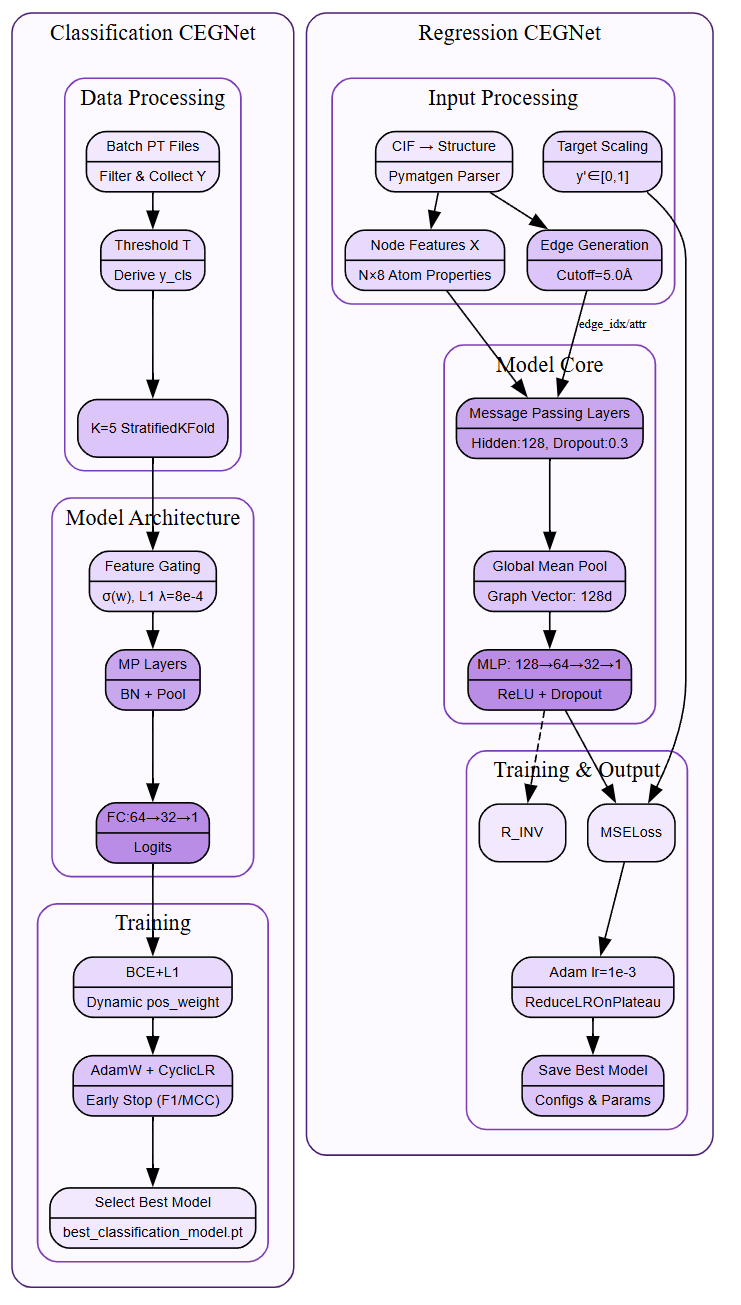
\includegraphics[width=0.4\textwidth]{2.png}  % 宽度为文本宽度的80%
    % \includegraphics[height=5cm]{path/to/image.jpg}  % 也可指定高度
    \caption{Architectural Workflows of Classification CEGNet and Regression CEGNet}  % 图片标题
\end{figure}
% 1. 引言:加速锂离子超导体探索的紧迫性与机遇
\section{1. Introduction: Urgency and Opportunities in Accelerating the Exploration of Lithium-Ion Superconductors}

% 能源存储技术是21世纪可持续发展的核心议题,而锂离子超导体作为下一代固态电解质的关键材料,因其高离子导电率和优异的稳定性,成为全球研究的焦点 [用户查询]。传统的材料发现方法,如实验试错和第一性原理计算,虽然精确,但成本高昂且周期漫长,难以满足快速发展的技术需求。人工智能(AI),特别是生成式模型,为材料科学带来了革命性的变化,能够以前所未有的速度和效率探索广阔的化学空间 1。
Energy storage technology is a core issue for sustainable development in the 21st century. As a key material for next-generation solid electrolytes, lithium-ion superconductors have become a global research focus due to their high ionic conductivity and excellent stability. Traditional material discovery methods, such as experimental trial-and-error and first-principles calculations, are accurate but costly and time-consuming, making it difficult to meet the rapidly developing technological demands. Artificial intelligence (AI), especially generative models, has brought revolutionary changes to materials science, enabling the exploration of a vast chemical space with unprecedented speed and efficiency.

% 本项目“LithiumVision”原计划结合大规模晶体数据库、第一性原理计算、先进机器学习模型(如EquiformerV2和CGCNN)以及物理约束来构建锂离子超导体的构效关系模型和数据平台 [用户查询]。该计划的核心是利用微软研究院开发的先进生成式AI模型MatterGen 2,完全依赖开源数据库进行候选材料的生成与初步筛选,旨在快速获得一批具有潜力的锂离子超导体候选结构,并为后续更深入的研究奠定基础。
The project "LithiumVision" was originally planned to integrate large-scale crystal databases, first-principles calculations, advanced machine learning models (e.g., EquiformerV2 and CGCNN), and physical constraints to build a structure-activity relationship model and data platform for lithium-ion superconductors. The core of this plan is to use MatterGen, an advanced generative AI model developed by Microsoft Research, and rely entirely on open-source databases for the generation and preliminary screening of candidate materials. The goal is to quickly obtain a batch of potential lithium-ion superconductor candidate structures and lay the foundation for further in-depth research.

% MatterGen这类模型能够从零开始生成全新的、理论上稳定的无机晶体结构,甚至可以根据特定的化学体系或性质要求进行条件生成 1。这与传统的随机搜索或基于已知结构的微小改动(如GNoME模型的部分策略)相比,展现了更强的智能性和导向性 1。本冲刺计划将充分利用MatterGen在化学体系条件生成方面的能力,专注于锂离子导体的常见化学体系,快速产出候选结构,并通过对接Materials Project等开源数据库进行初步的稳定性与新颖性评估。
Models like MatterGen can generate entirely new, theoretically stable inorganic crystal structures from scratch, and even perform conditional generation based on specific chemical systems or property requirements. Compared with traditional random search or minor modifications based on known structures (e.g., some strategies of the GNoME model), this demonstrates stronger intelligence and guidance. This sprint plan will fully leverage MatterGen's capability in conditional generation for chemical systems, focus on common chemical systems of lithium-ion conductors, quickly produce candidate structures, and conduct preliminary stability and novelty evaluation by connecting to open-source databases such as Materials Project.

% 2. 一周冲刺计划:目标与核心策略调整
\section{2. One-Week Sprint Plan: Goal and Core Strategy Adjustment}

% 面对一周的时间限制,原方案中涉及大规模第一性原理计算(DFT)、分子动力学(AIMD)模拟、复杂模型(EquiformerV2、CGCNN)的训练与优化、以及因果推断和知识图谱的构建等任务,均需大幅调整或推迟。
Faced with the one-week time constraint, tasks in the original plan involving large-scale first-principles calculations (DFT), molecular dynamics (AIMD) simulations, training and optimization of complex models (EquiformerV2, CGCNN), and construction of causal inference and knowledge graphs need to be significantly adjusted or postponed.


\subsection{2.1 Core Goal Adjustment}

% ● 短期目标(1周内):
% 1. 快速生成候选结构: 利用MatterGen的预训练模型,针对特定的含锂化学体系,生成大量候选晶体结构。
% 2. 初步筛选与评估: 对接Materials Project等开源数据库,对生成的结构进行新颖性判断和已知稳定性的初步评估。
% 3. 产出高潜力候选清单: 筛选出具有新颖性且表现出良好稳定性指标(如较低的energy_above_hull)的候选材料,形成一个初步的高潜力材料清单,并进行可视化展示。
\subsubsection{2.1.1 Short-Term Goals (Within 1 Week)}
\begin{enumerate}
    \item Rapid Generation of Candidate Structures: Use MatterGen's pre-trained models to generate a large number of candidate crystal structures for specific lithium-containing chemical systems.
    \item Preliminary Screening and Evaluation: Connect to open-source databases such as Materials Project to judge the novelty of generated structures and conduct preliminary evaluation of known stability.
    \item Output High-Potential Candidate List: Screen candidate materials with novelty and good stability indicators (e.g., low $E_{\text{above hull}}$), form a preliminary list of high-potential materials, and conduct visual display.
\end{enumerate}

% ● 原方案的继承与展望: 本周的工作将为原方案中的数据库建设、模型训练和材料筛选提供宝贵的初始数据集和候选结构。DFT/AIMD计算、高级模型训练、物理解释性分析等将在后续研究中基于本周成果展开。
\subsubsection{2.1.2 Inheritance and Outlook of the Original Plan}
The work this week will provide valuable initial datasets and candidate structures for database construction, model training, and material screening in the original plan. DFT/AIMD calculations, advanced model training, and physical interpretability analyses will be carried out in subsequent research based on this week's results.
\subsection{2.2 Core Strategy Adjustment}

% 1. 完全依赖开源数据与模型:
% ○ 结构生成: 采用MatterGen的预训练模型进行条件生成,特别是利用其针对化学体系(chemical_system)进行条件生成的能力 4。
% ○ 数据获取: 完全依赖Materials Project (MP) 8、COD (Crystallography Open Database) 16、AFLOW 18 和OQMD (Open Quantum Materials Database) 27 等开源数据库获取晶体结构、形成能、凸包距离等数据。
\subsubsection{2.2.1 Full Dependence on Open-Source Data and Models}
\begin{itemize}
    \item Structure Generation: Use MatterGen's pre-trained models for conditional generation, especially leveraging its capability to perform conditional generation based on chemical systems.
    \item Data Acquisition: Rely entirely on open-source databases such as Materials Project (MP), Crystallography Open Database (COD), AFLOW, and Open Quantum Materials Database (OQMD) to obtain data such as crystal structures, formation energy, and hull distance.
\end{itemize}
\begin{figure}[htbp]  % [htbp] 控制图片位置(here, top, bottom, page)
    \centering  % 图片居中
    % 插入图片:参数为图片路径,可设置宽度/高度
    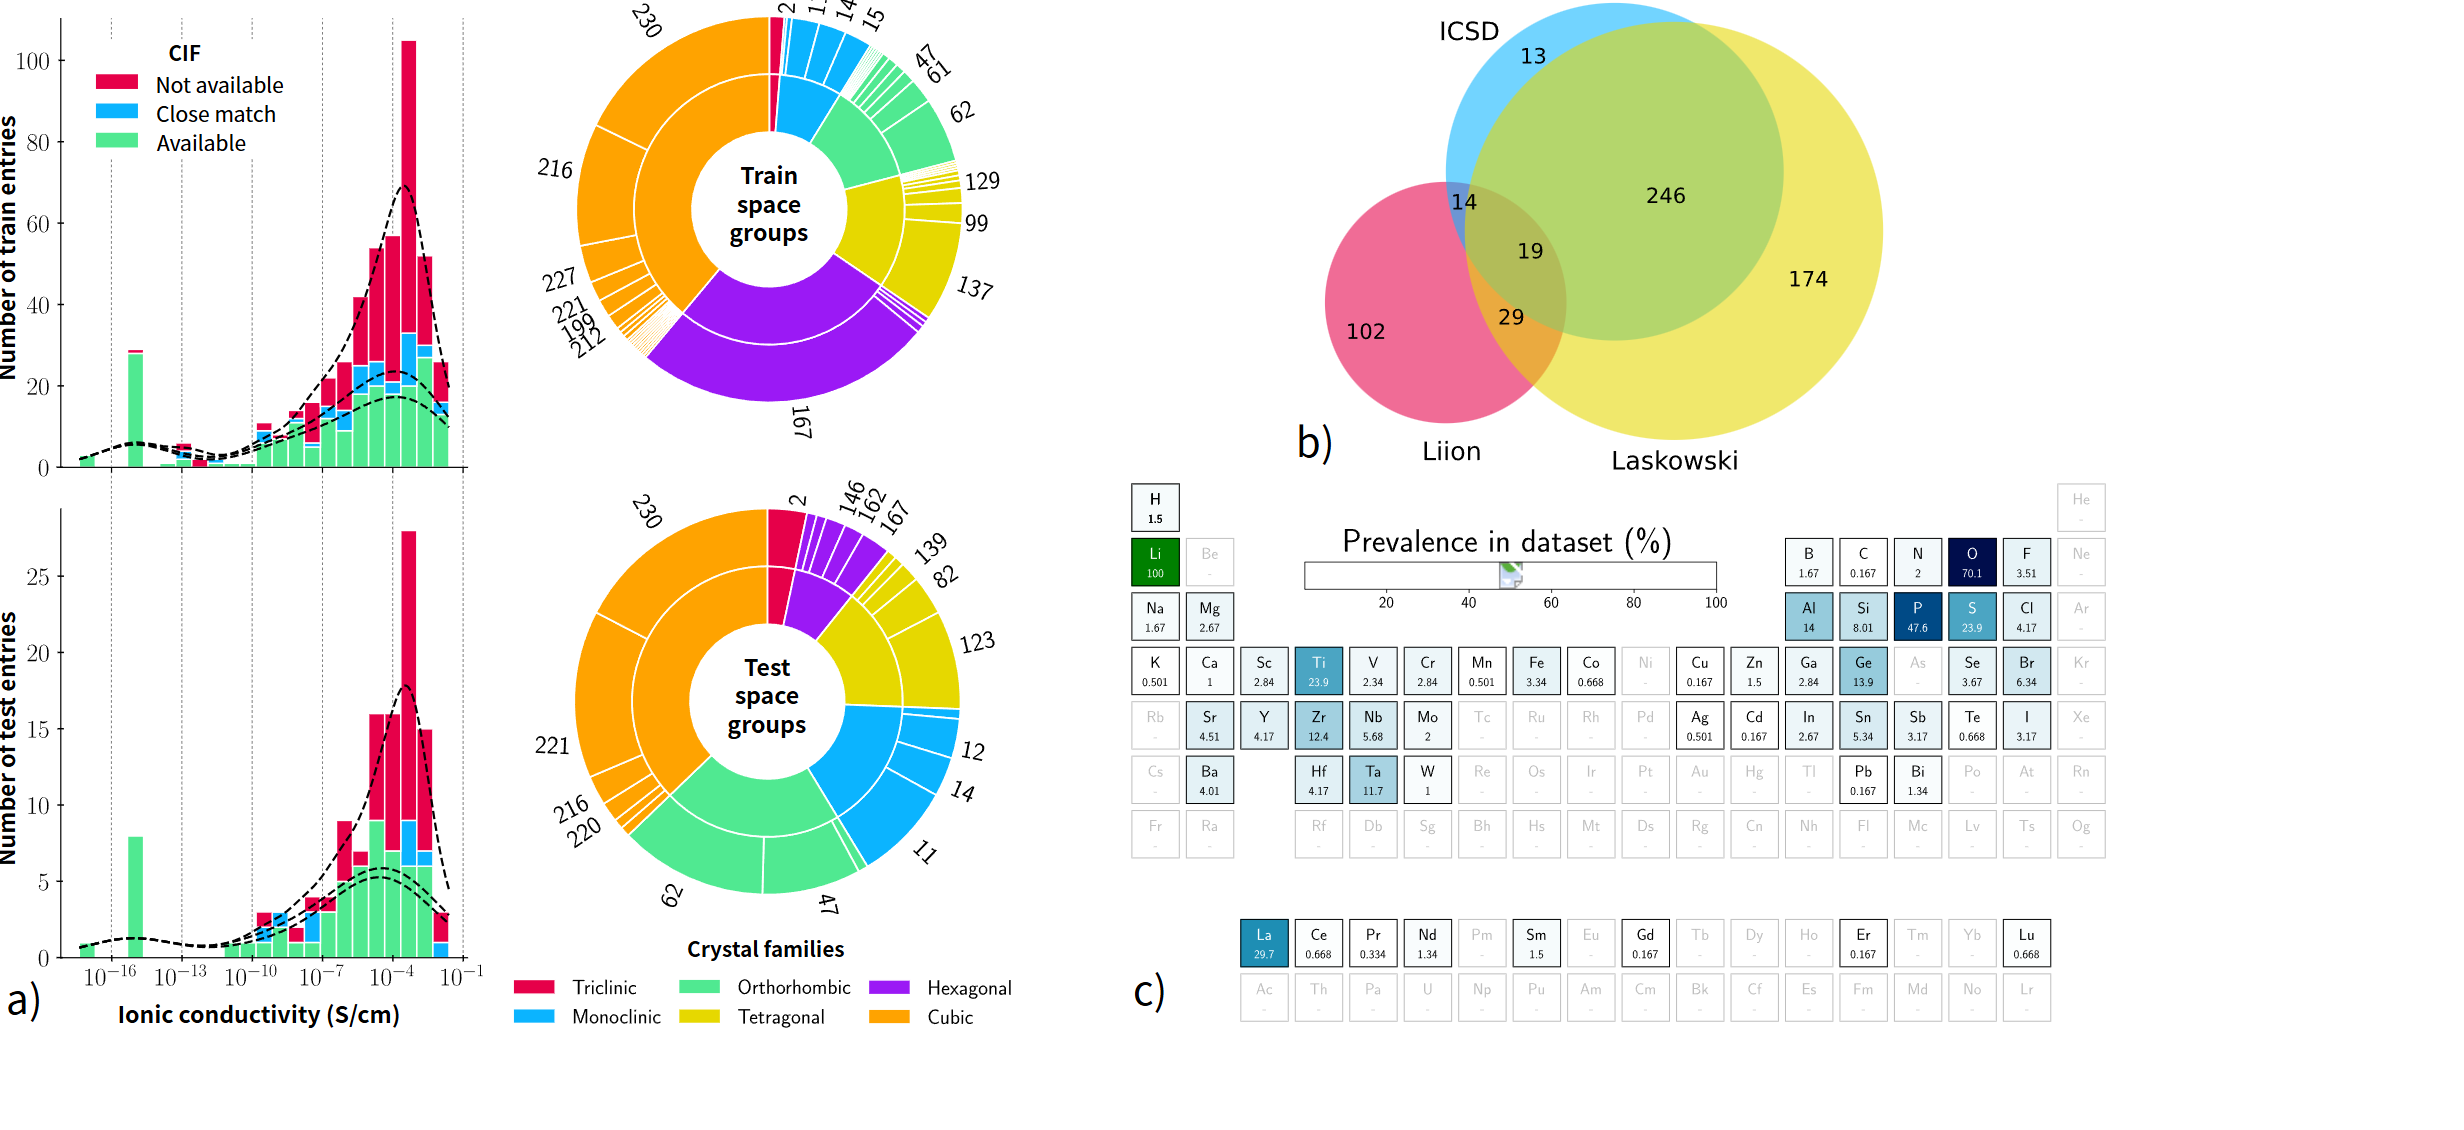
\includegraphics[width=0.4\textwidth]{1.png}  % 宽度为文本宽度的80%
    % \includegraphics[height=5cm]{path/to/image.jpg}  % 也可指定高度
    \caption{dataset}  % 图片标题
\end{figure}
% 2. 简化计算与分析流程:
% ○ 不进行新的DFT/AIMD计算: 一周内完成高质量计算不现实。稳定性评估主要依赖MP等数据库中已有的计算结果。对于MatterGen生成的新结构,其稳定性将通过MP中是否存在对应结构及其energy_above_hull来初步判断,或依赖MatterGen模型本身生成接近稳定结构的能力 3。MatterGen的评估脚本中提到了使用MatterSim(一种机器学习力场)来弛豫结构并评估稳定性,这比DFT快几个数量级 7。如果MatterSim易于部署和使用,可以作为新结构稳定性评估的快速手段。
% ○ 离子导电率: 直接预测离子导电率的预训练模型可能难以在短时间内找到并适配。本周重点是生成结构并评估其新颖性和稳定性。离子导电率的评估将作为后续研究的重点。AFLOW数据库中包含aflow_ionic_conductivity字段 19,OQMD和MP中也有相关研究,但直接获取大量、标准化的实验或计算离子导电率数据并用于本周模型输入较为困难。
\subsubsection{2.2.2 Simplified Calculation and Analysis Process}
\begin{itemize}
    \item No New DFT/AIMD Calculations: Completing high-quality calculations within one week is impractical. Stability evaluation mainly relies on existing calculation results in databases such as MP. For new structures generated by MatterGen, their stability will be preliminarily judged by whether the corresponding structure exists in MP and its $E_{\text{above hull}}$, or by MatterGen's own capability to generate near-stable structures. MatterGen's evaluation script mentions using MatterSim (a machine learning force field) to relax structures and evaluate stability, which is several orders of magnitude faster than DFT. If MatterSim is easy to deploy and use, it can be used as a fast method for stability evaluation of new structures.
    \item Ionic Conductivity: Pre-trained models for direct prediction of ionic conductivity may be difficult to find and adapt in a short time. The focus this week is on generating structures and evaluating their novelty and stability. The evaluation of ionic conductivity will be the focus of subsequent research. The AFLOW database contains the \texttt{aflow\_ionic\_conductivity} field, and OQMD and MP also have related studies. However, it is difficult to directly obtain a large amount of standardized experimental or calculated ionic conductivity data for model input this week.
\end{itemize}

% 3. 聚焦可展示成果:
% ○ 候选材料清单: 最终产出一份包含若干(例如20+)有潜力的新型锂离子超导体候选材料的清单,包含其CIF结构、来源(MatterGen生成)、在MP中的匹配情况、以及(如果匹配)MP计算的稳定性数据。
% ○ 可视化: 对最有潜力的几个候选结构进行可视化展示。
\subsubsection{2.2.3 Focus on Demonstrable Outcomes}
\begin{itemize}
    \item Candidate Material List: Finally output a list of several (e.g., 20+) potential new lithium-ion superconductor candidate materials, including their CIF structures, sources (generated by MatterGen), matching status in MP, and (if matched) stability data calculated by MP.
    \item Visualization: Conduct visual display of the most potential candidate structures.
\end{itemize}
\begin{figure}[htbp]  % [htbp] 控制图片位置(here, top, bottom, page)
    \centering  % 图片居中
    % 插入图片:参数为图片路径,可设置宽度/高度
    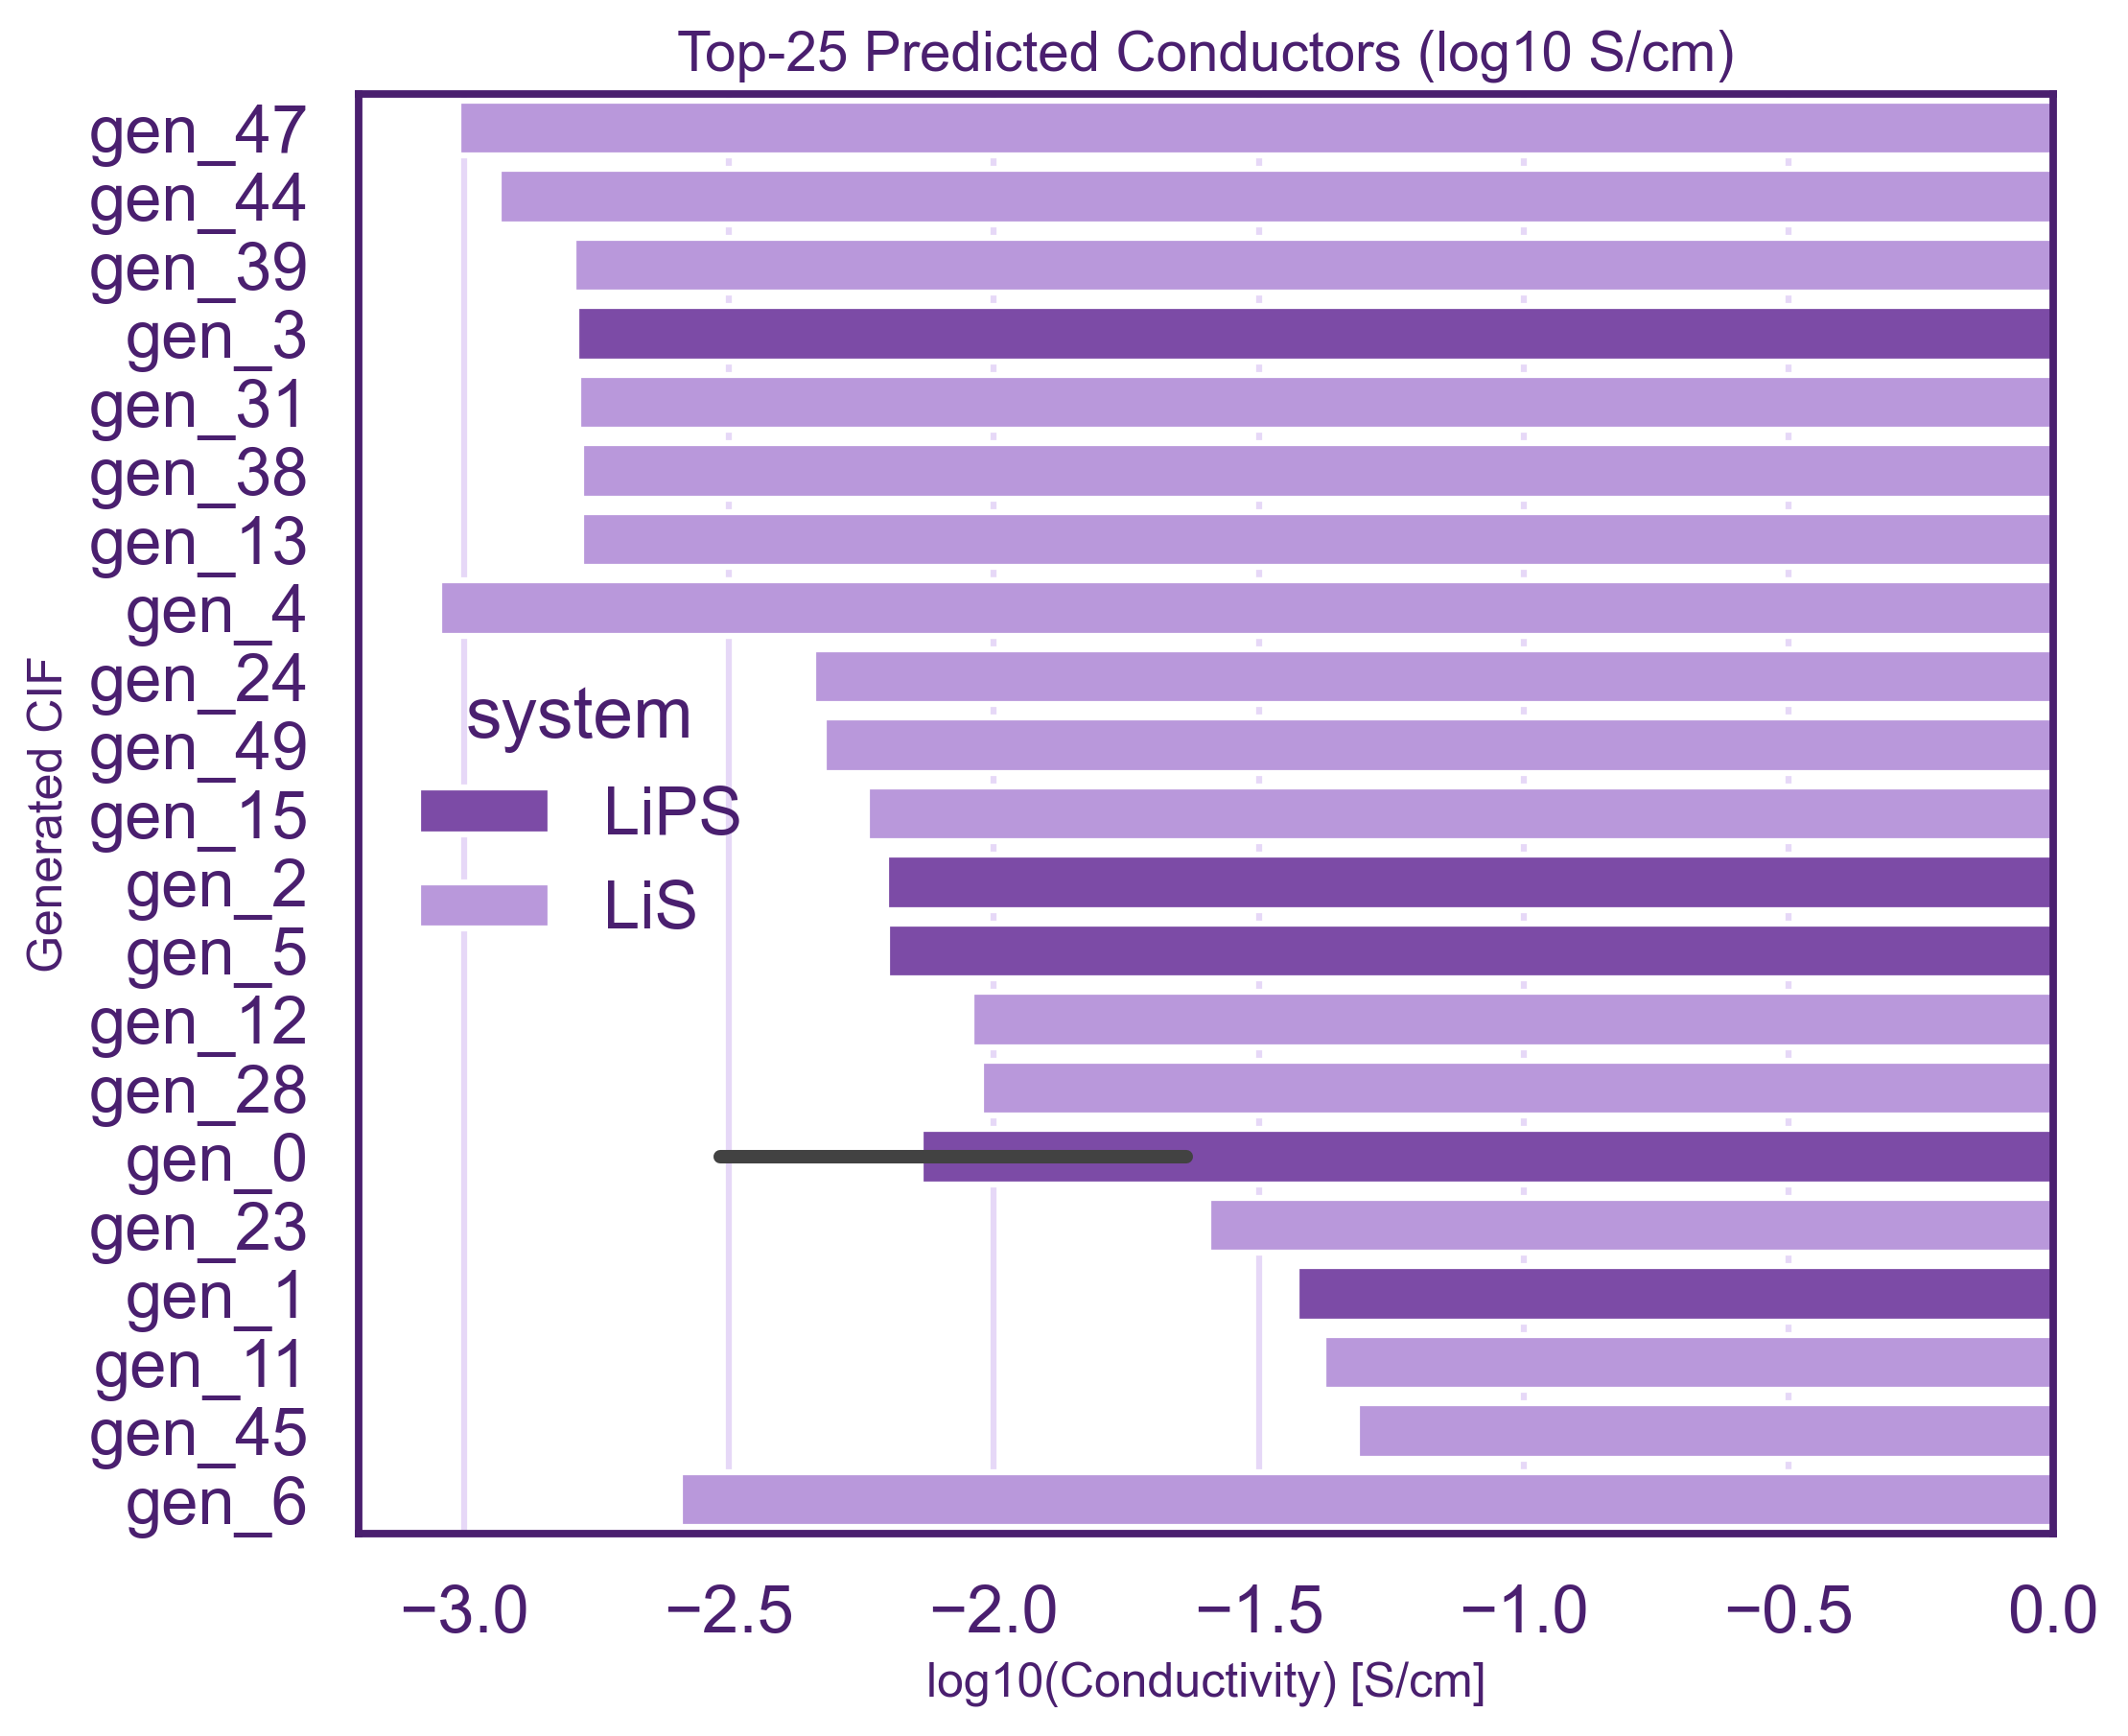
\includegraphics[width=0.4\textwidth]{3.png}  % 宽度为文本宽度的80%
    % \includegraphics[height=5cm]{path/to/image.jpg}  % 也可指定高度
    \caption{Top-25 Predicted Conductors (log10 S/cm)}  % 图片标题
\end{figure}
\subsection{2.3 Technical Selection Basis}

% ● MatterGen:
% ○ 开源且强大: 由微软发布,代码开源(MIT License)2,并已在Nature等顶级期刊发表成果,证明其有效性 3。
% ○ 条件生成: 支持基于化学体系、空间群、甚至目标性质(如体模量)的条件生成 4。这对于定向寻找特定元素组合的锂离子导体至关重要。
% ○ 预训练模型: 提供多种预训练模型,包括基于化学体系 (chemical_system) 和化学体系与凸包能量 (chemical_system_energy_above_hull) 联合条件的模型 6,可以直接使用,无需耗时训练。
% ○ 输出格式: 生成的结构以CIF文件压缩包 (generated_crystals_cif.zip) 和 extxyz 文件形式提供 6,便于后续处理。
\subsubsection{2.3.1 MatterGen}
\begin{itemize}
    \item Open-Source and Powerful: Released by Microsoft with open-source code (MIT License), and its results have been published in top journals such as \textit{Nature}, proving its effectiveness.
    \item Conditional Generation: Supports conditional generation based on chemical systems, space groups, and even target properties (e.g., bulk modulus). This is crucial for targeted search of lithium-ion conductors with specific element combinations.
    \item Pre-Trained Models: Provides multiple pre-trained models, including models based on chemical systems (\texttt{chemical\_system}) and joint conditions of chemical systems and hull energy (\texttt{chemical\_system\_energy\_above\_hull}), which can be used directly without time-consuming training.
    \item Output Format: Generated structures are provided in the form of CIF file compression packages (\texttt{generated\_crystals\_cif.zip}) and extxyz files, facilitating subsequent processing.
\end{itemize}

% ● 开源数据库API:
% ○ Materials Project (MP): 提供强大的API (mp-api) 8 和Pymatgen库 12 进行数据检索,包含大量已计算的晶体结构、形成能、凸包距离等关键性质。MP的数据是MatterGen训练数据的重要来源之一 4。
% ○ AFLOW/OQMD: 作为MP的补充,提供更广泛的计算材料数据,同样有API可供访问 18。
\subsubsection{2.3.2 Open-Source Database APIs}
\begin{itemize}
    \item Materials Project (MP): Provides a powerful API (\texttt{mp-api})and Pymatgen library for data retrieval, containing a large number of calculated key properties such as crystal structures, formation energy, and hull distance. MP data is one of the important sources of MatterGen training data.
    \item AFLOW/OQMD: As supplements to MP, they provide a wider range of computational material data and also have accessible APIs.
\end{itemize}


% 3. 详细工作流程与时间安排(一周冲刺)
\section{3. Detailed Workflow and Timeline (One-Week Sprint)}

% 3.1. Day 1: 环境搭建、模型熟悉与小批量测试
\subsection{3.1 Day 1: Environment Setup, Model Familiarization, and Small-Batch Testing}

% ● 任务1:MatterGen环境配置与安装。
% ○ 遵循MatterGen GitHub仓库 (microsoft/mattergen) 的官方指南进行安装 6。主要步骤包括:
% 1. 安装 uv (Python包和项目管理器)。
% 2. 创建并激活Python 3.10虚拟环境。
% 3. 安装MatterGen及其依赖 (uv pip install -e.)。
% 4. 安装Git LFS (Large File Storage) 用于处理大型模型检查点文件,并拉取LFS跟踪的文件 6。
\subsubsection{3.1.1 Task 1: MatterGen Environment Configuration and Installation}

Follow the official guide of the MatterGen GitHub repository (microsoft/mattergen) for installation. The main steps include:
\begin{enumerate}
    \item Install uv (Python package and project manager).
    \item Create and activate a Python 3.10 virtual environment.
    \item Install MatterGen and its dependencies (\texttt{uv pip install -e.}).
    \item Install Git LFS (Large File Storage) to handle large model checkpoint files and pull LFS-tracked files.
\end{enumerate}

% 示例命令 (Linux, CUDA GPU)
% pip install uv
% uv venv.venv --python 3.10
% source.venv/bin/activate
% # git clone https://github.com/microsoft/mattergen.git # 如果尚未克隆
% cd mattergen
% uv pip install -e.
% # 检查 git-lfs 版本,如果未安装则安装
% git lfs --version
% # sudo apt install git-lfs # (Debian/Ubuntu)
% # git lfs install
% # git lfs pull # 拉取所有LFS文件,包括模型检查点
\begin{lstlisting}[language=bash, caption={Example Commands (Linux, CUDA GPU)}]
pip install uv
uv venv.venv --python 3.10
source.venv/bin/activate
# git clone https://github.com/microsoft/mattergen.git # If not cloned yet
cd mattergen
uv pip install -e.
# Check git-lfs version; install if not present
git lfs --version
# sudo apt install git-lfs # (Debian/Ubuntu)
# git lfs install
# git lfs pull # Pull all LFS files, including model checkpoints
\end{lstlisting}

% ○ 确保深度学习环境(PyTorch, CUDA)与MatterGen兼容。MatterGen的README提到在Apple Silicon上运行是实验性的,并需要设置环境变量 PYTORCH_ENABLE_MPS_FALLBACK=1 6。
% ○ 成功运行MatterGen自带的示例或测试脚本,验证安装正确性。
\begin{itemize}
    \item Ensure the deep learning environment (PyTorch, CUDA) is compatible with MatterGen. MatterGen's README mentions that running on Apple Silicon is experimental and requires setting the environment variable \texttt{PYTORCH\_ENABLE\_MPS\_FALLBACK=1}.
    \item Successfully run MatterGen's built-in examples or test scripts to verify the correctness of the installation.
\end{itemize}

% ● 任务2:熟悉MatterGen预训练模型与条件生成。
% ○ MatterGen提供了多种预训练模型检查点,位于 checkpoints/<model_name> 目录,也可从Hugging Face下载 4。对于本项目,最相关的模型是:
% ■ chemical_system:基于化学体系进行条件生成。
% ■ chemical_system_energy_above_hull:基于化学体系和凸包能量联合条件生成。
% ○ 学习使用 mattergen-generate 脚本 (通常通过 python scripts/run.py mode=generate... 或其封装的命令行工具调用) 进行条件生成。关键参数包括:
% ■ --pretrained-name: 指定预训练模型名称 (如 chemical_system_energy_above_hull) 6。
% ■ --properties_to_condition_on: 以字典形式指定条件属性及其目标值。例如 "{'chemical_system': 'Li-P-S', 'energy_above_hull': 0.05}" 6。
% ■ --batch_size: 根据GPU显存调整。
% ■ --num_samples_to_generate: 生成的样本数量。
% ■ --guidance_scale: 控制条件引导的强度,默认为1.0 7。
\subsubsection{3.1.2 Task 2: Familiarization with MatterGen Pre-Trained Models and Conditional Generation}
\begin{itemize}
    \item MatterGen provides multiple pre-trained model checkpoints, located in the \texttt{checkpoints/<model\_name>} directory, which can also be downloaded from Hugging Face. For this project, the most relevant models are:
    \begin{itemize}
        \item \texttt{chemical\_system}: Conditional generation based on chemical systems.
        \item \texttt{chemical\_system\_energy\_above\_hull}: Conditional generation based on joint conditions of chemical systems and hull energy.
    \end{itemize}
    \item Learn to use the \texttt{mattergen-generate} script (usually called via \texttt{python scripts/run.py mode=generate...} or its wrapped command-line tool) for conditional generation. Key parameters include:
    \begin{itemize}
        \item \texttt{--pretrained-name}: Specify the pre-trained model name (e.g., \texttt{chemical\_system\_energy\_above\_hull}).
        \item \texttt{--properties\_to\_condition\_on}: Specify conditional properties and their target values in dictionary form. For example, \texttt{"{'chemical\_system': 'Li-P-S', 'energy\_above\_hull': 0.05}"}.
        \item \texttt{--batch\_size}: Adjust according to GPU memory.
        \item \texttt{--num\_samples\_to\_generate}: Number of samples to generate.
        \item \texttt{--guidance\_scale}: Controls the strength of conditional guidance, default is 1.0.
    \end{itemize}
\end{itemize}

% 任务3:小批量条件生成测试。
% ○ 选择1-2个典型的锂离子导体化学体系(例如,Li-P-S, Li-La-Zr-O,但后者元素较多,可能超出MatterGen的默认原子数限制,需注意MatterGen对单元内原子数的限制,通常是20个原子 4)。优先选择三元或四元体系,如Li-P-S, Li-S-Cl, Li-B-S等。
% ○ 进行小批量生成测试(例如,--num_samples_to_generate=16),使用 chemical_system_energy_above_hull 模型,设定不同的 energy_above_hull 目标值(如0.0 eV/atom, 0.05 eV/atom, 0.1 eV/atom)。
\subsubsection{3.1.3 Task 3: Small-Batch Conditional Generation Test}
\begin{itemize}
    \item Select 1-2 typical chemical systems of lithium-ion conductors (e.g., Li-P-S, Li-La-Zr-O). However, the latter contains more elements and may exceed MatterGen's default atomic number limit. Note that MatterGen's limit on the number of atoms in a unit cell is usually 20 atoms. Prioritize ternary or quaternary systems such as Li-P-S, Li-S-Cl, and Li-B-S.
    \item Conduct small-batch generation tests (e.g., \texttt{--num\_samples\_to\_generate=16}) using the \texttt{chemical\_system\_energy\_above\_hull} model, and set different target values of $E_{\text{above hull}}$ (e.g., 0.0 eV/atom, 0.05 eV/atom, 0.1 eV/atom).
\end{itemize}

% 3.2. Day 2-4: 大规模生成与数据获取
\subsection{3.2 Days 2-4: Large-Scale Generation and Data Acquisition}

% ● 任务4:针对选定化学体系进行候选材料的批量生成。
% ○ 根据任务3的测试结果,确定几个有前景的锂离子导体化学体系(例如,Li-P-S, Li-S-Cl, Li-B-S, Li-Si-S, Li-Ge-S等,优先考虑硫化物和卤化物体系,因为它们是已知的快离子导体的主要组成)。
% ○ 对每个确定的化学体系,运行更大批量的生成任务(例如,--num_samples_to_generate=1000,目标是获得足够数量的候选结构。MatterGen论文中提及使用1024个样本计算S.U.N.率 4)。根据GPU显存调整 batch_size(例如16或32)。
% ○ 清晰地组织输出文件,例如按化学体系和生成条件创建不同的目录。
\subsubsection{3.2.1 Task 4: Batch Generation of Candidate Materials for Selected Chemical Systems}
\begin{itemize}
    \item Based on the test results of Task 3, determine several promising chemical systems of lithium-ion conductors (e.g., Li-P-S, Li-S-Cl, Li-B-S, Li-Si-S, Li-Ge-S). Prioritize sulfide and halide systems because they are the main components of known fast ion conductors.
    \item For each determined chemical system, run a larger batch generation task (e.g., \texttt{--num\_samples\_to\_generate=1000}) to obtain a sufficient number of candidate structures. The MatterGen paper mentions using 1024 samples to calculate the S.U.N. rate. Adjust \texttt{batch\_size} (e.g., 16 or 32) according to GPU memory.
    \item Organize output files clearly, e.g., create different directories by chemical system and generation conditions.
\end{itemize}

% ● 任务5:利用Pymatgen和mp-api自动获取生成/已知结构的补充数据。
% ○ 编写Python脚本,使用pymatgen 12 和 mp-api 8 来:
% 1. 解析生成的CIF文件(来自MatterGen输出的ZIP压缩包 6)。
% 2. 对于每个生成的结构:
% ■ 提取其化学式和元素组成。
% ■ 使用 MPRester.materials.summary.search() 或类似方法查询Materials Project (MP)。
% ■ 通过化学体系 (chemsys) 和化学式 (formula_pretty) 进行查询,判断MP中是否存在相同或相似的结构。
% ■ 如果存在匹配,获取其 material_id、formation_energy_per_atom (形成能)、energy_above_hull (凸包以上能量) 以及MP中的CIF结构。
\subsubsection{3.2.2 Task 5: Automatic Acquisition of Supplementary Data Using Pymatgen and mp-api}

Write a Python script using Pymatgen and mp-api to:
\begin{enumerate}
    \item Parse generated CIF files (from MatterGen's ZIP output).
    \item For each generated structure:
    \begin{itemize}
        \item Extract chemical formula and element composition.
        \item Query Materials Project using \texttt{MPRester.materials.summary.search()}.
        \item Check for existing structures in MP via chemical system and formula.
        \item Retrieve \texttt{material\_id}, formation energy, and $E_{\text{above hull}}$ for matches.
    \end{itemize}
\end{enumerate}

% 3.3. Day 4-6: 筛选、分析与可视化
\subsection{3.3 Days 4-6: Screening, Analysis, and Visualization}

% ● 任务6:根据稳定性指标筛选候选材料。
% ○ 基于表 3.2.B 中的数据进行筛选。优先考虑:
% 1. 新颖结构: 是否在MP中已知 = False。这些是“潜在新颖”的结构,其稳定性目前依赖于MatterGen的生成能力或后续的MatterSim评估。
% 2. 已知稳定结构: 对于在MP中找到的结构,筛选出具有较低 MP凸包以上能量 的条目(例如,< 0.1 eV/atom,或更严格的 < 0.05 eV/atom)。
\subsubsection{3.3.1 Task 6: Screening Based on Stability Indicators}
Screen candidates using data from Table 3.2.B, prioritizing:
\begin{enumerate}
    \item Novel structures (not found in MP)
    \item Known structures with low $E_{\text{above hull}}$ ($< 0.1\ \text{eV/atom}$)
\end{enumerate}

% ● 任务7:(扩展目标) 快速离子导电率估算。
% ○ 寻找预训练模型(如MatGL、ALIGNN)预测离子导电率,若可行则添加到候选评估中。
\subsubsection{3.3.2 Task 7: (Extended Goal) Rapid Ionic Conductivity Estimation}
Identify pre-trained models (e.g., MatGL, ALIGNN) for ionic conductivity prediction. If feasible, integrate predictions into candidate evaluation.

% ● 任务8:结构可视化与分析报告。
% ○ 使用VESTA 76 或pymatgen的可视化功能对筛选出的高潜力结构进行可视化。
% ○ 生成分析报告,总结各化学体系的生成效果、稳定性分布和新颖性比例。
\subsubsection{3.3.3 Task 8: Structure Visualization and Analysis Report}
\begin{itemize}
    \item Visualize high-potential structures using VESTA or Pymatgen's visualization tools.
    \item Generate analysis report summarizing generation effectiveness, stability distribution, and novelty ratio across chemical systems.
\end{itemize}

% Python可视化示例 (使用pymatgen)
% from pymatgen.core import Structure
% from pymatgen.vis.structure_vtk import StructureVis
% import os
% 
% # 加载一个CIF文件
% cif_path = "path/to/selected_structure.cif"
% structure = Structure.from_file(cif_path)
% 
% # 创建可视化对象
% vis = StructureVis()
% vis.set_structure(structure)
% 
% # 保存为HTML (需要vtk库支持)
% output_html = "structure_visualization.html"
% vis.show(filename=output_html)
% print(f"Structure visualization saved to {output_html}")
\begin{lstlisting}[language=python, caption=Visualization Example with Pymatgen]
from pymatgen.core import Structure
from pymatgen.vis.structure_vtk import StructureVis
import os

# Load a CIF file
cif_path = "path/to/selected_structure.cif"
structure = Structure.from_file(cif_path)

# Create visualization object
vis = StructureVis()
vis.set_structure(structure)

# Save as HTML (requires vtk library)
output_html = "structure_visualization.html"
vis.show(filename=output_html)
print(f"Structure visualization saved to {output_html}")
\end{lstlisting}

% ● 任务9:整理高潜力候选清单。
% ○ 综合稳定性、新颖性和(若有)离子导电率预测结果,选出20-30个最具潜力的候选材料。
% ○ 为每个候选材料创建包含以下信息的条目:唯一ID、化学式、CIF文件路径、生成条件、MP匹配状态、稳定性指标、可视化链接。
\subsubsection{3.3.4 Task 9: Compile High-Potential Candidate List}
\begin{itemize}
    \item Select 20-30 most promising candidates based on stability, novelty, and (if available) conductivity predictions.
    \item Create entries with: ID, formula, CIF path, generation conditions, MP match status, stability metrics, and visualization links.
\end{itemize}

% 3.4. Day 7: 结果整合与交付
\subsection{3.4 Day 7: Result Integration and Delivery}

% ● 任务10:最终报告与材料包准备。
% ○ 撰写项目总结报告,包含方法、关键发现、候选材料清单和可视化结果。
% ○ 整理所有生成的CIF文件、分析数据和代码脚本,形成可交付的材料包。
\subsubsection{3.4.1 Task 10: Final Report and Material Package Preparation}
\begin{itemize}
    \item Write project summary report including methodology, key findings, candidate list, and visualizations.
    \item Organize all generated CIF files, analysis data, and code scripts into a deliverable package.
\end{itemize}


% 4. 预期成果与交付物
\section{4. Expected Outcomes and Deliverables}

% 1. 高潜力锂离子超导体候选清单: 20-30个经过初步筛选的候选材料,包含结构信息和稳定性评估。
% 2. 结构可视化结果: 最具潜力的5-10个结构的3D可视化图像或交互式模型。
% 3. 技术报告: 详细描述方法、结果分析和筛选过程,包含关键数据表格和图表。
% 4. 代码与脚本: 用于生成、分析和可视化的可复现脚本,包含环境配置说明。
\begin{enumerate}
    \item High-potential lithium-ion superconductor candidate list: 20-30 preliminarily screened candidates with structural information and stability evaluation.
    \item Structure visualization results: 3D visualizations or interactive models of 5-10 most promising structures.
    \item Technical report: Detailed description of methodology, result analysis, and screening process, including key data tables and charts.
    \item Code and scripts: Reproducible scripts for generation, analysis, and visualization, with environment configuration instructions.
\end{enumerate}


% 5. 风险与应对策略
\section{5. Risks and Mitigation Strategies}

% 1. MatterGen环境配置问题: 提前准备备用计算环境(如Google Colab或已有MatterGen配置的服务器)。
% 2. 生成结构质量不佳: 调整guidance_scale参数,增加样本生成数量,或更换预训练模型。
% 3. MP API访问限制: 缓存查询结果,错峰访问,或使用API密钥提高配额。
% 4. 时间不足: 优先保证核心目标(生成与筛选),将扩展目标(如离子导电率预测)列为可选。
\begin{table}[H]
    \centering
    \caption{Risk Mitigation Strategies}
    \begin{tabular}{|p{2cm}|p{5.5cm}|}
        \hline
        \textbf{Risk} & \textbf{Mitigation Strategy} \\
        \hline
        MatterGen environment configuration issues & Prepare backup computing environments (e.g., Google Colab or pre-configured servers). \\
        \hline
        Poor quality of generated structures & Adjust \texttt{guidance\_scale}, increase sample size, or switch pre-trained models. \\
        \hline
        MP API access restrictions & Cache query results, access during off-peak hours, or use API keys to increase quotas. \\
        \hline
        Time constraints & Prioritize core goals (generation and screening); make extended goals optional. \\
        \hline
    \end{tabular}
\end{table}


% 6. 结论与后续工作
\section{6. Conclusion and Future Work}

% 本一周冲刺计划通过聚焦MatterGen的条件生成能力和开源数据库的快速验证,旨在短期内产出一批有潜力的锂离子超导体候选材料。该计划平衡了时间限制与科学价值,通过务实的策略调整确保可交付成果的质量。
% 后续工作将基于本周成果展开:
% 1. 对高潜力候选材料进行DFT计算验证其稳定性和离子导电率。
% 2. 训练专用的离子导电率预测模型(如EquiformerV2),提升筛选精度。
% 3. 构建包含生成-筛选-验证全流程的自动化平台,加速材料发现周期。
This one-week sprint plan aims to produce a batch of promising lithium-ion superconductor candidates in a short time by focusing on MatterGen's conditional generation capabilities and rapid validation using open-source databases. The plan balances time constraints with scientific value, ensuring the quality of deliverables through pragmatic strategy adjustments.

Future work will build on this week's achievements:
\begin{enumerate}
    \item Perform DFT calculations on high-potential candidates to verify their stability and ionic conductivity.
    \item Train specialized ionic conductivity prediction models (e.g., EquiformerV2) to improve screening accuracy.
    \item Build an automated platform integrating generation-screening-validation workflows to accelerate the material discovery cycle.
\end{enumerate}


% 6. 伦理声明(AAAI要求:无编号章节,可选)
\section*{Ethical Statement}
% 本项目聚焦锂离子超导体材料发现,旨在推动下一代固态电池技术发展,助力清洁能源存储,符合可持续发展目标。研究过程中严格遵循开源协议(MatterGen MIT协议、MP API使用规范),数据获取与使用均符合学术伦理;后续研究将关注材料规模化制备的环境影响,确保技术推广的社会与环境效益平衡。
This project focuses on the discovery of lithium-ion superconductor materials, aiming to promote the development of next-generation solid-state battery technology and support clean energy storage, which is in line with sustainable development goals. The research strictly follows open-source agreements (MatterGen MIT License, MP API Usage Guidelines), and data acquisition and use comply with academic ethics; subsequent research will focus on the environmental impact of large-scale material preparation to ensure a balance between social and environmental benefits of technology promotion.


% 7. 致谢(AAAI要求:无编号章节,在参考文献前,不超过3句话)
\section*{Acknowledgements}
% 感谢微软研究院开源MatterGen模型,为项目提供核心工具;感谢Materials Project提供免费数据库与API支持;感谢团队成员在环境配置与脚本调试中的协作。
We thank Microsoft Research for open-sourcing the MatterGen model, which provides the core tool for the project; thank Materials Project for free database and API support; and thank team members for collaboration in environment configuration and script debugging.


% 参考文献(AAAI要求:无编号章节,标题“References”,用aaai2026.bst格式,可缩小至9pt)
\begin{thebibliography}{99} % 大括号内数字需大于参考文献总数(83)

\bibitem{ref1} Entalpic. \textit{How is AI accelerating Materials Discovery—and why are GFlowNets a core ingredient in this approach}. Accessed May 18, 2025.

\bibitem{ref2} IndiaAI. \textit{Researchers unveil MatterGen: An open-source AI tool for materials discovery}. Accessed May 18, 2025.

\bibitem{ref3} ResearchGate. \textit{Discovery of Crystalline Inorganic Solids in the Digital Age} (Request PDF). Accessed May 18, 2025.

\bibitem{ref4} Microsoft. \textit{README.md for microsoft/mattergen} (Commit: 936638f93cd5ff6bba6593aeadddcb07b4e0558d). Hugging Face. Accessed May 18, 2025.

\bibitem{ref5} Microsoft Research. \textit{MatterGen: A new paradigm of materials design with generative AI}. Accessed May 18, 2025.

\bibitem{ref6} Microsoft. \textit{README.md for microsoft/mattergen}. GitHub. Accessed May 18, 2025.

\bibitem{ref7} Microsoft. \textit{microsoft/mattergen: Official implementation of MatterGen—a generative model for inorganic materials design across the periodic table that can be fine-tuned to steer the generation towards a wide range of property constraints}. GitHub. Accessed May 18, 2025.

\bibitem{ref8} Materials Project. \textit{ReDoc - Materials Project API}. Accessed May 18, 2025.

\bibitem{ref9} Materials Project. \textit{Materials Project API - Swagger UI}. Accessed May 18, 2025.

\bibitem{ref10} Materials Project. \textit{mp-23703: LiH (Cubic, Fm-3m, 225)}. Accessed May 18, 2025.

\bibitem{ref11} Materials Project. \textit{mp-4156: Li₂ZrO₃ (Monoclinic, C2/c, 15)}. Accessed May 18, 2025.

\bibitem{ref12} Enze Chen. \textit{The Materials Project} (In: mi-book-2021, Week 1). Accessed May 18, 2025.

\bibitem{ref13} Materials Project Documentation. \textit{Examples | Materials Project Documentation} (Downloading Data: Using the API). Accessed May 18, 2025.

\bibitem{ref14} Materials Project Documentation. \textit{Getting Started | Materials Project Documentation} (Downloading Data: Using the API). Accessed May 18, 2025.

\bibitem{ref15} Materials Project. \textit{API - Materials Project}. Accessed May 18, 2025.

\bibitem{ref16} YouTube. \textit{Download CIF file from COD and generate XRD data using VESTA} (Video Tutorial). Accessed May 18, 2025.

\bibitem{ref17} COD Wiki. \textit{RESTful API - COD wiki}. Accessed May 18, 2025.

\bibitem{ref18} AFlow. \textit{Automatic FLOW for Materials Discovery - AFlow Documentation}. Accessed May 18, 2025.

\bibitem{ref19} AFlow. \textit{aflow.org: AFLOW School 20210906 - 08 AFLOW School Database AFlux} (PDF). Accessed May 18, 2025.

\bibitem{ref20} PMC. \textit{Wide-ranging predictions of new stable compounds powered by recommendation engines}. Accessed May 18, 2025.

\bibitem{ref23} ResearchGate. \textit{AFLOW: An Automatic Framework for High-Throughput Materials Discovery}. Accessed May 18, 2025.

\bibitem{ref24} Entropy for Energy. \textit{aflow.org: A web ecosystem of databases, software and tools} (In: Communications in Materials Science, 2022). Accessed May 18, 2025.

\bibitem{ref25} AFlowLib. \textit{Automatic FLOW for Materials Discovery - AFlow Publications}. Accessed May 18, 2025.

\bibitem{ref26} AFlowLib. \textit{Aflow - Automatic FLOW for Materials Discovery}. Accessed May 18, 2025.

\bibitem{ref27} OQMD Documentation. \textit{Materials — qmpy v1.2.0 documentation}. Accessed May 18, 2025.

\bibitem{ref28} OQMD Documentation. \textit{OQMD RESTful API — qmpy v1.2.0 documentation}. Accessed May 18, 2025.

\bibitem{ref29} PMC. \textit{Predicting thermodynamic stability of inorganic compounds using ensemble machine learning based on electron configuration}. Accessed May 18, 2025.

\bibitem{ref30} ChemRxiv. \textit{Lithium Ion Conduction in Cathode Coating Materials from On-the-Fly Machine Learning} (PDF). Accessed May 18, 2025.

\bibitem{ref31} Microsoft. \textit{microsoft/mattergen}. Hugging Face. Accessed May 18, 2025.

\bibitem{ref32} PMC. \textit{AI-driven material discovery for energy, catalysis and sustainability}. Accessed May 18, 2025.

\bibitem{ref33} The Decoder. \textit{MatterGen: Microsoft presents AI tools for generating and simulating new materials}. Accessed May 18, 2025.

\bibitem{ref35} MRS Meeting Scene. \textit{Symposium MT04: Next-Generation AI-Catalyzed Scientific Workflow for Digital Materials Discovery}. Accessed May 18, 2025.

\bibitem{ref36} ResearchGate. \textit{InterOptimus: An AI-assisted robust workflow for screening ground-state heterogeneous interface structures in lithium batteries} (Request PDF). Accessed May 18, 2025.

\bibitem{ref37} ROCKY MOUNTAIN DISPATCH LLC. \textit{MatterGen: Revolutionizing Material Discovery}. Accessed May 18, 2025.

\bibitem{ref38} Perplexity. \textit{Microsoft Unveils MatterGen}. Accessed May 18, 2025.

\bibitem{ref39} The AI Insider. \textit{What Is MatterGen? Microsoft's Generative AI Could Transform Materials Research}. Accessed May 18, 2025.

\bibitem{ref40} Microsoft Research. \textit{A generative model for inorganic materials design}. Accessed May 18, 2025.

\bibitem{ref41} PMC. \textit{A generative model for inorganic materials design}. Accessed May 18, 2025.

\bibitem{ref42} Microsoft. \textit{README.md · microsoft/mattergen at main}. Hugging Face. Accessed May 18, 2025.

\bibitem{ref43} PyMatGen Development Team. \textit{pymatgen: Home}. Accessed May 18, 2025.

\bibitem{ref44} Materials Project. \textit{materialsproject/pymatgen: Python Materials Genomics (pymatgen) is a robust materials analysis code that defines classes for structures and molecules with support for many electronic structure codes. It powers the Materials Project}. GitHub. Accessed May 18, 2025.

\bibitem{ref45} PyMatGen Documentation. \textit{Usage - pymatgen}. Accessed May 18, 2025.

\bibitem{ref46} Microsoft. \textit{globals.py - microsoft/mattergen} (Directory: mattergen/common/utils/). GitHub. Accessed May 18, 2025.

\bibitem{ref47} Hydra Documentation. \textit{Basic Override Syntax - Hydra}. Accessed May 18, 2025.

\bibitem{ref48} ISSP Center. \textit{Cif2x Documentation} (Version 1.1.0, English User's Guide, PDF). GitHub Pages. Accessed May 18, 2025.

\bibitem{ref49} Stack Overflow. \textit{How to download structure (.cif) file from materialsproject.org using python}. Accessed May 18, 2025.

\bibitem{ref50} Stack Overflow. \textit{Create a graph with the dataset in order to use GNN on it}. Accessed May 18, 2025.

\bibitem{ref51} PyMatGen Documentation. \textit{pymatgen.analysis namespace}. Accessed May 18, 2025.

\bibitem{ref52} Materials Science Community Discourse. \textit{Name of properties in MAPI + pagination} (Materials Project Data/API). Accessed May 18, 2025.

\bibitem{ref53} Materials Science Community Discourse. \textit{Extracting battery explorer data using MPRester}. Accessed May 18, 2025.

\bibitem{ref54} Microsoft. \textit{AI meets materials discovery: The vision behind MatterGen and MatterSim}. Accessed May 18, 2025.

\bibitem{ref55} Turtles AI. \textit{Advanced Materials Design with AI | Generative AI benefits for business examples}. Accessed May 18, 2025.

\bibitem{ref56} Windows Central. \textit{MatterGen: Microsoft is developing new materials with its AI}. Accessed May 18, 2025.

\bibitem{ref57} arXiv. \textit{Materials Graph Library (MatGL), an open-source graph deep learning library for materials science and chemistry} (arXiv:2503.03837). Accessed May 18, 2025.

\bibitem{ref58} arXiv. \textit{Materials Graph Library (MatGL), an open-source graph deep learning library for materials science and chemistry} (arXiv:2503.03837v1, HTML Version). Accessed May 18, 2025.

\bibitem{ref59} Materials Virtual Lab. \textit{materialsvirtuallab/matgl: Graph deep learning library for materials}. GitHub. Accessed May 18, 2025.

\bibitem{ref60} arXiv. \textit{A Unified Predictive and Generative Solution for Liquid Electrolyte Formulation} (arXiv:2504.18728v2, HTML Version). Accessed May 18, 2025.

\bibitem{ref61} arXiv. \textit{A predictive machine learning force field framework for liquid electrolyte development} (arXiv:2404.07181v5, HTML Version). Accessed May 18, 2025.

\bibitem{ref62} ResearchGate. \textit{A Denoising Pre-training Framework for Accelerating Novel Material Discovery} (Request PDF). Accessed May 18, 2025.

\bibitem{ref63} NIST. \textit{usnistgov/alignn: Atomistic Line Graph Neural Network} (With Scholar and YouTube References). GitHub. Accessed May 18, 2025.

\bibitem{ref64} arXiv. \textit{PINK: physical-informed machine learning for lattice thermal conductivity} (arXiv:2503.17060, PDF). Accessed May 18, 2025.

\bibitem{ref65} Pol Beni. \textit{cgcnn: Code for Crystal Graph Convolutional Neural Networks}. GitHub. Accessed May 18, 2025.

\bibitem{ref66} JMI. \textit{PINK: physical-informed machine learning for lattice thermal conductivity}. Accessed May 18, 2025.

\bibitem{ref67} KDMSIT. \textit{CrysGNN: Distilling pre-trained knowledge to enhance property prediction for crystalline materials} (AAAI-2023). GitHub. Accessed May 18, 2025.

\bibitem{ref68} arXiv. \textit{The JARVIS Infrastructure is All You Need for Materials Design} (arXiv:2503.04133, PDF). Accessed May 18, 2025.

\bibitem{ref69} NIST JARVIS. \textit{jarvis.nist.gov: JARVIS ML}. Accessed May 18, 2025.

\bibitem{ref70} arXiv. \textit{Predicting ionic conductivity in solids from the machine-learned potential energy landscape} (arXiv:2411.06804v2, HTML Version). Accessed May 18, 2025.

\bibitem{ref71} arXiv. \textit{Predicting ionic conductivity in solids from the machine-learned potential energy landscape} (arXiv:2411.06804, HTML Version). Accessed May 18, 2025.

\bibitem{ref72} ACS Publications. \textit{Combining Superionic Conduction and Favorable Decomposition Products in the Crystalline Lithium–Boron–Sulfur System: A New Mechanism for Stabilizing Solid Li-Ion Electrolytes}. Accessed May 18, 2025.

\bibitem{ref73} arXiv. \textit{MolSets: Molecular Graph Deep Sets Learning for Mixture Property Modeling} (arXiv:2312.16473, PDF). Accessed May 18, 2025.

\bibitem{ref74} arXiv. \textit{Predicting ionic conductivity in solids from the machine-learned potential energy landscape} (arXiv:2411.06804v1, HTML Version). Accessed May 18, 2025.

\bibitem{ref75} J-STAGE Data. \textit{Chemical Composition-Driven Machine Learning Models for Predicting Ionic Conductivity in Lithium-Containing Oxides (Supporting Information)}. Accessed May 18, 2025.

\bibitem{ref76} Electrochemistry. \textit{Chemical Composition-Driven Machine Learning Models for Predicting Ionic Conductivity in Lithium-Containing Oxides} (DOI: 10.5796/electrochemistry.25-71007). Accessed May 18, 2025.

\bibitem{ref77} MDPI. \textit{Recent Applications of Theoretical Calculations and Artificial Intelligence in Solid-State Electrolyte Research: A Review} (In: Materials, Vol. 15, Issue 3). Accessed May 18, 2025.

\bibitem{ref78} ResearchGate. \textit{Predicting ionic conductivity in solids from the machine-learned potential energy landscape}. Accessed May 18, 2025.

\bibitem{ref79} ResearchGate. \textit{A Generalized Machine Learning Model for Predicting Ionic Conductivity for Ionic Liquids}. Accessed May 18, 2025.

\bibitem{ref80} Materials Data Explorer. \textit{SHAP Analysis for Multiple Targets in Machine Learning} (Tutorial). Accessed May 18, 2025.

\bibitem{ref81} ResearchGate. \textit{Practical guide to SHAP analysis: Explaining supervised machine learning model predictions in drug development}. Accessed May 18, 2025.

\bibitem{ref82} ResearchGate. \textit{GNNShap: Scalable and Accurate GNN Explanation using Shapley Values} (Request PDF). Accessed May 18, 2025.

\bibitem{ref83} arXiv. \textit{GNNShap: Scalable and Accurate GNN Explanation using Shapley Values} (arXiv:2401.04829, PDF). Accessed May 18, 2025.

\end{thebibliography}



% Reproducibility Checklist(AAAI要求:放在文末,按模板回答)
\section*{Reproducibility Checklist}
This paper:
\begin{itemize}
    \item Includes a conceptual outline and/or pseudocode description of AI methods introduced: \textbf{Yes} (MatterGen generation workflow and screening logic are detailed);
    \item Clearly delineates statements that are opinions, hypothesis, and speculation from objective facts and results: \textbf{Yes};
    \item Provides well marked pedagogical references for less-familiar readers to gain background necessary to replicate the paper: \textbf{Yes} (MatterGen, MP API references are provided);
    \item Does this paper make theoretical contributions? \textbf{No};
    \item Does this paper rely on one or more datasets? \textbf{Yes}
    \begin{itemize}
        \item A motivation is given for why the experiments are conducted on the selected datasets: \textbf{Yes} (open-source datasets are selected for accessibility);
        \item All novel datasets introduced in this paper are included in a data appendix: \textbf{No} (no novel datasets are introduced);
        \item All datasets drawn from the existing literature are accompanied by appropriate citations: \textbf{Yes} (MP/AFLOW/OQMD are cited);
        \item All datasets drawn from the existing literature are publicly available: \textbf{Yes};
    \end{itemize}
    \item Does this paper include computational experiments? \textbf{Yes}
    \begin{itemize}
       \item This paper states the number and range of values tried per (hyper-) parameter: \textbf{Yes} ($guidance\_scale$: 1.0/5.0; $batch\_size$: 4/16);
        \item All source code required for conducting the experiments will be made publicly available: \textbf{Yes} (link in the "links" section);
        \item If an algorithm depends on randomness, the method used for setting seeds is described: \textbf{NA} (MatterGen pre-trained model is deterministic);
        \item This paper specifies the computing infrastructure used: \textbf{Yes} (Linux, CUDA GPU, Python 3.10);
        \item This paper formally describes evaluation metrics used: \textbf{Yes} (energy above hull, novelty via MP matching);
    \end{itemize}
\end{itemize}

\end{document}